\section{Discussion}\label{sec:discussion}
\subsection{Snell's Law}
\paragraph{Task 4}\textit{Compare the angles of incidence, reflection and transmission in an air $\rightarrow \epsilon_r = 2$ and $\epsilon_r = 2 \rightarrow $air interface.}
\begin{figure}[htpb]
	\subfigure[$\epsilon_r = 1 \rightarrow \epsilon_r = 2$]
	{
		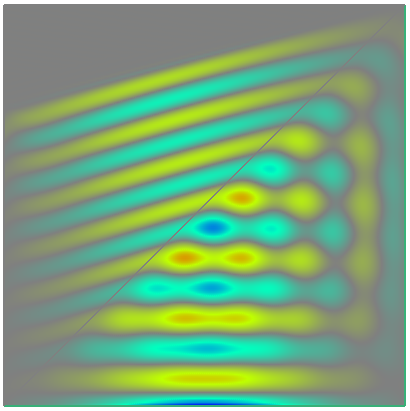
\includegraphics[width=0.475\linewidth]{graphics/Task2-1-to-2}
	}
	\subfigure[$\epsilon_r = 2 \rightarrow \epsilon_r = 1$]
	{
		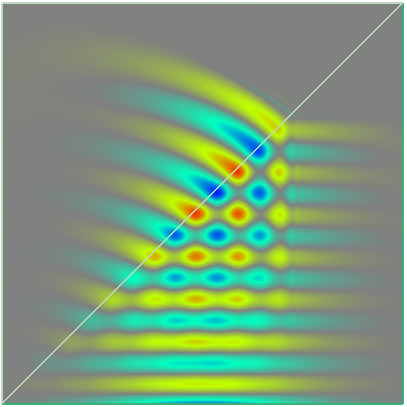
\includegraphics[width=0.475\linewidth]{graphics/Task4-2-to-1}
	}
	\caption{Behavior at \SI{45}{\degree} incidence}
	\label{fig:snell}
\end{figure}

\todo[inline]{Compute the angles of reflection and transmission}

\paragraph{Task 6}\textit{Compare the images for $\epsilon_r$ = 2.0, 2.5, 3.0 in the ABC-bounded region.}

\begin{figure}[htpb]
	\subfigure[$\epsilon_r = 2.5 \rightarrow \epsilon_r = 1$]
	{
		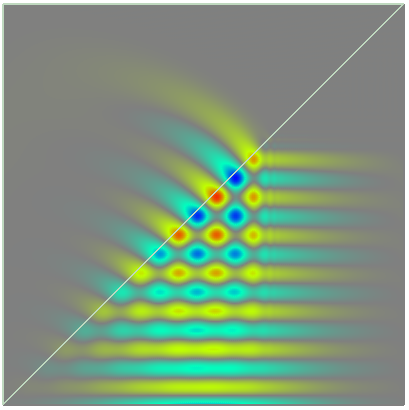
\includegraphics[width=0.475\linewidth]{graphics/Task5-2,5-to-1}
	}
	\subfigure[$\epsilon_r = 3 \rightarrow \epsilon_r = 1$]
	{
		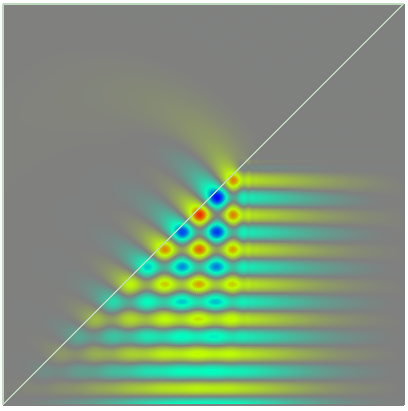
\includegraphics[width=0.475\linewidth]{graphics/Task6-3-to-1}
	}
	\caption{Behavior at \SI{45}{\degree} incidence}
	\label{fig:TIR}
\end{figure}

\todo[inline]{Compute the TIR angles for the 2, 2.5, 3 to 1 interface.}
\todo[inline]{Why does the ``spray'' into the second medium decrease as $\epsilon_r$ increases?}

\paragraph{Task 8}\textit{Capture an animation of \vect{H} with pointer mode and comment on it.}

\begin{figure}[tbph]
	\centering
	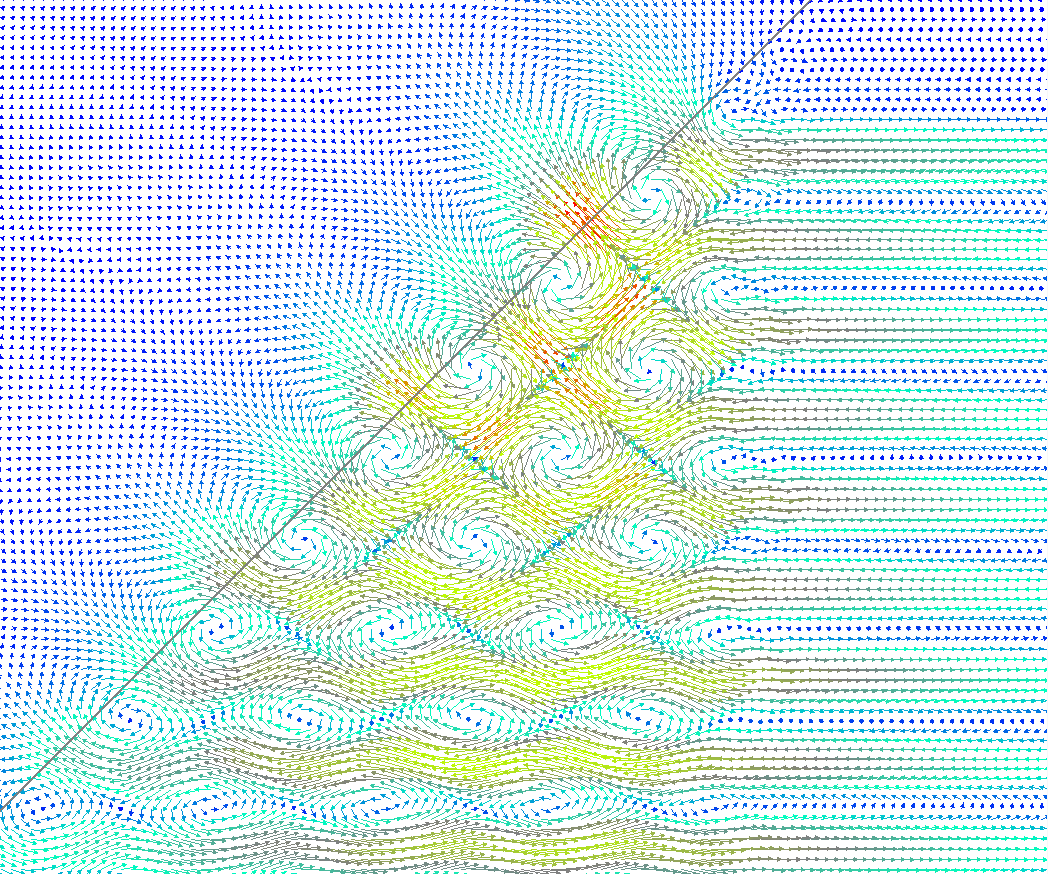
\includegraphics[width=0.8\linewidth]{graphics/Task8-Pointers}
	\caption{\vect{H} for $\epsilon_r = 3 \rightarrow \epsilon_r = 1$}
	\label{fig:Task8-Pointers}
\end{figure}

As \vect{E} is reflected by the boundary it creates a standing wave, perpendicular to the plane of Fig.~\ref{fig:Task8-Pointers}.
As per Ampere's Law, \vect{H} curls around the perpendicular \vect{E} field, creating the ``pools'' in the image. 

Fig.~\ref{fig:Task8-Pointers-Inset} shows that \vect{H} is not altered by the boundary.
\begin{figure}[tbph]
	\centering
	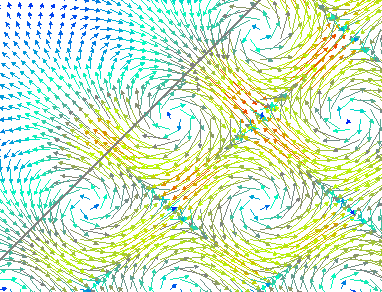
\includegraphics[width=0.6\linewidth]{graphics/Task8-Pointers-Inset}
	\caption{Inset view of Fig.~\ref{fig:Task8-Pointers}}
	\label{fig:Task8-Pointers-Inset}
\end{figure}
Since \vect{E} was reflected by the boundary, \vect{H} dissipates because it is not able to generate itself in isolation.

\subsection{Brewster angle}
\paragraph{Task 9}\textit{Design a Brewster angle interface for zero reflection transmission of a plane wave from air to a dielectric with $\epsilon_r = 4$.}
The Brewster angle for this interface is:
\begin{align*}
	\tan\theta_B = \sqrt{{\epsilon_2 \over \epsilon_1}} \implies \theta_B = \tan^{-1}(2) = \SI{63.435}{\degree} 
\end{align*}
The second medium is designed with a base of 200 mm and height of 400 mm to ensure an incidence angle of $\theta_B$.
This is shown in Fig.~\ref{fig:Task9-Brewster}.

\begin{figure}[tbph]
	\centering
	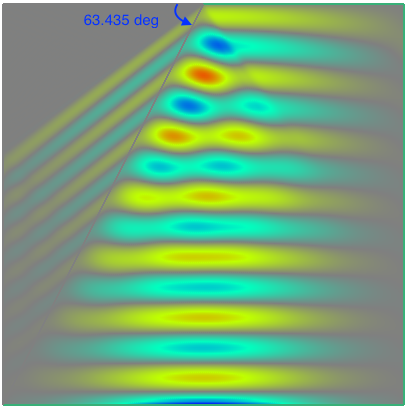
\includegraphics[width=0.6\linewidth]{graphics/Task9-Brewster}
	\caption{A Brewster angle interface}
	\label{fig:Task9-Brewster}
\end{figure}


\subsection{Rectangular waveguides and cavities}
\paragraph{Task 16}\textit{Obtain the resonant frequencies of the constructed waveguide and compare it to the calculated values.}

Fig.~\ref{fig:Task16-Analyzer} shows the response generated by the impulse function.
\begin{figure}[tbph]
	\centering
	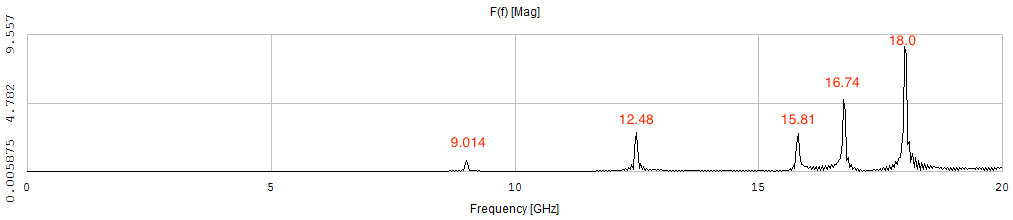
\includegraphics[width=0.95\linewidth]{graphics/Task16-Analyzer-annotated}
	\caption{Frequency response of waveguide}
	\label{fig:Task16-Analyzer}
\end{figure}

For $TE_{11}$, the cutoff frequency is:
\begin{align*}
	f_c = {u_{p0} \over 2} \sqrt{\left({m \over a}\right)^2 + \left({n \over b}\right)^2} = {c_0 \over 2} \sqrt{\left({1 \over \SI{30}{\milli\meter}}\right)^2 + \left({1 \over \SI{20}{\milli\meter}}\right)^2} = \SI{9.007}{\giga\hertz}
\end{align*}
\todo[inline]{verify calculation}
This corresponds with the first peak of Fig.~\ref{fig:Task16-Analyzer}.


\subsection{Rectangular waveguide modes}
\paragraph{Task 20}\textit{Compare the propagation in a waveguide with $TE_{10}$ and $TE_{30}$.}

$TE_{30}$ has $f_c \approx \SI{4.5}{\giga\hertz}$.
Any frequency above this value with propagate through the waveguide, but significantly higher frequencies will generate the best graphics.
Fig.~\ref{fig:Task20-T30-50GHz} was generated with a source at \SI{50}{\giga\hertz}

\begin{figure}[tbph]
	\centering
	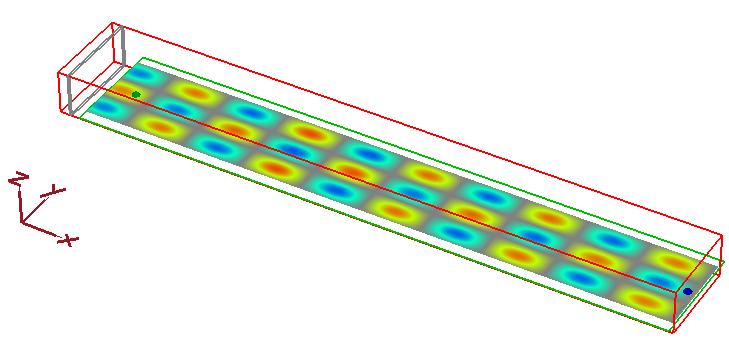
\includegraphics[width=0.7\linewidth]{graphics/Task20-T30-50GHz}
	\caption{Transmission in a $TE_{30}$ waveguide}
	\label{fig:Task20-T30-50GHz}
\end{figure}

